\section{Ablation Studies}

\subsection{Influence of Iterative Refinement on SFT Performance}

% \begin{table}[t]
% \centering
% \caption{Experiment results and computational costs for Llama-3-8B-Tulu models across multiple iterations.}
% \renewcommand{\arraystretch}{0.95}
% \resizebox{0.48\textwidth}{!}{
% \begin{tabular}{c|cc|cc|cc}
% \toprule
% \multirow{2}{*}{\textbf{Iteration}} & \multicolumn{2}{c|}{\textbf{FollowBench}} & \multicolumn{2}{c|}{\textbf{AlpacaEval2}} & \multicolumn{2}{c} {\textbf{Token Numbers}} 
% \\
% & \textbf{HSR}        & \textbf{SSR}       & \textbf{LC.}      & \textbf{Len} & \textbf{Input} & \textbf{Output} \\ 
% \midrule
% 1    & 49.75   & 64.78    & 21.63  & 1,994  & 1,882 & 1,869  \\
% 2   & 53.82    & 67.55    & 21.01     & 1,829   & 3,351 & 2,562   \\
% 3   & \textbf{54.46}        & 67.54     & 20.69   & 1,722      & 4,844 & 3,275   \\
% 4   & 53.97       & 67.09    & \textbf{22.50}      & 1,672      & 6,361 & 4,008   \\
% 5   & 53.30     & \textbf{67.91}    & 20.78    & 1,599    & 7,902 & 4,761  \\
% \bottomrule
% \end{tabular}}
% \label{table:judge_iterations}
% \end{table}

\begin{figure}[pos=htbp]
    \centering
    \includegraphics[width=0.48\textwidth]{source/SFT_iterations.png}
    % 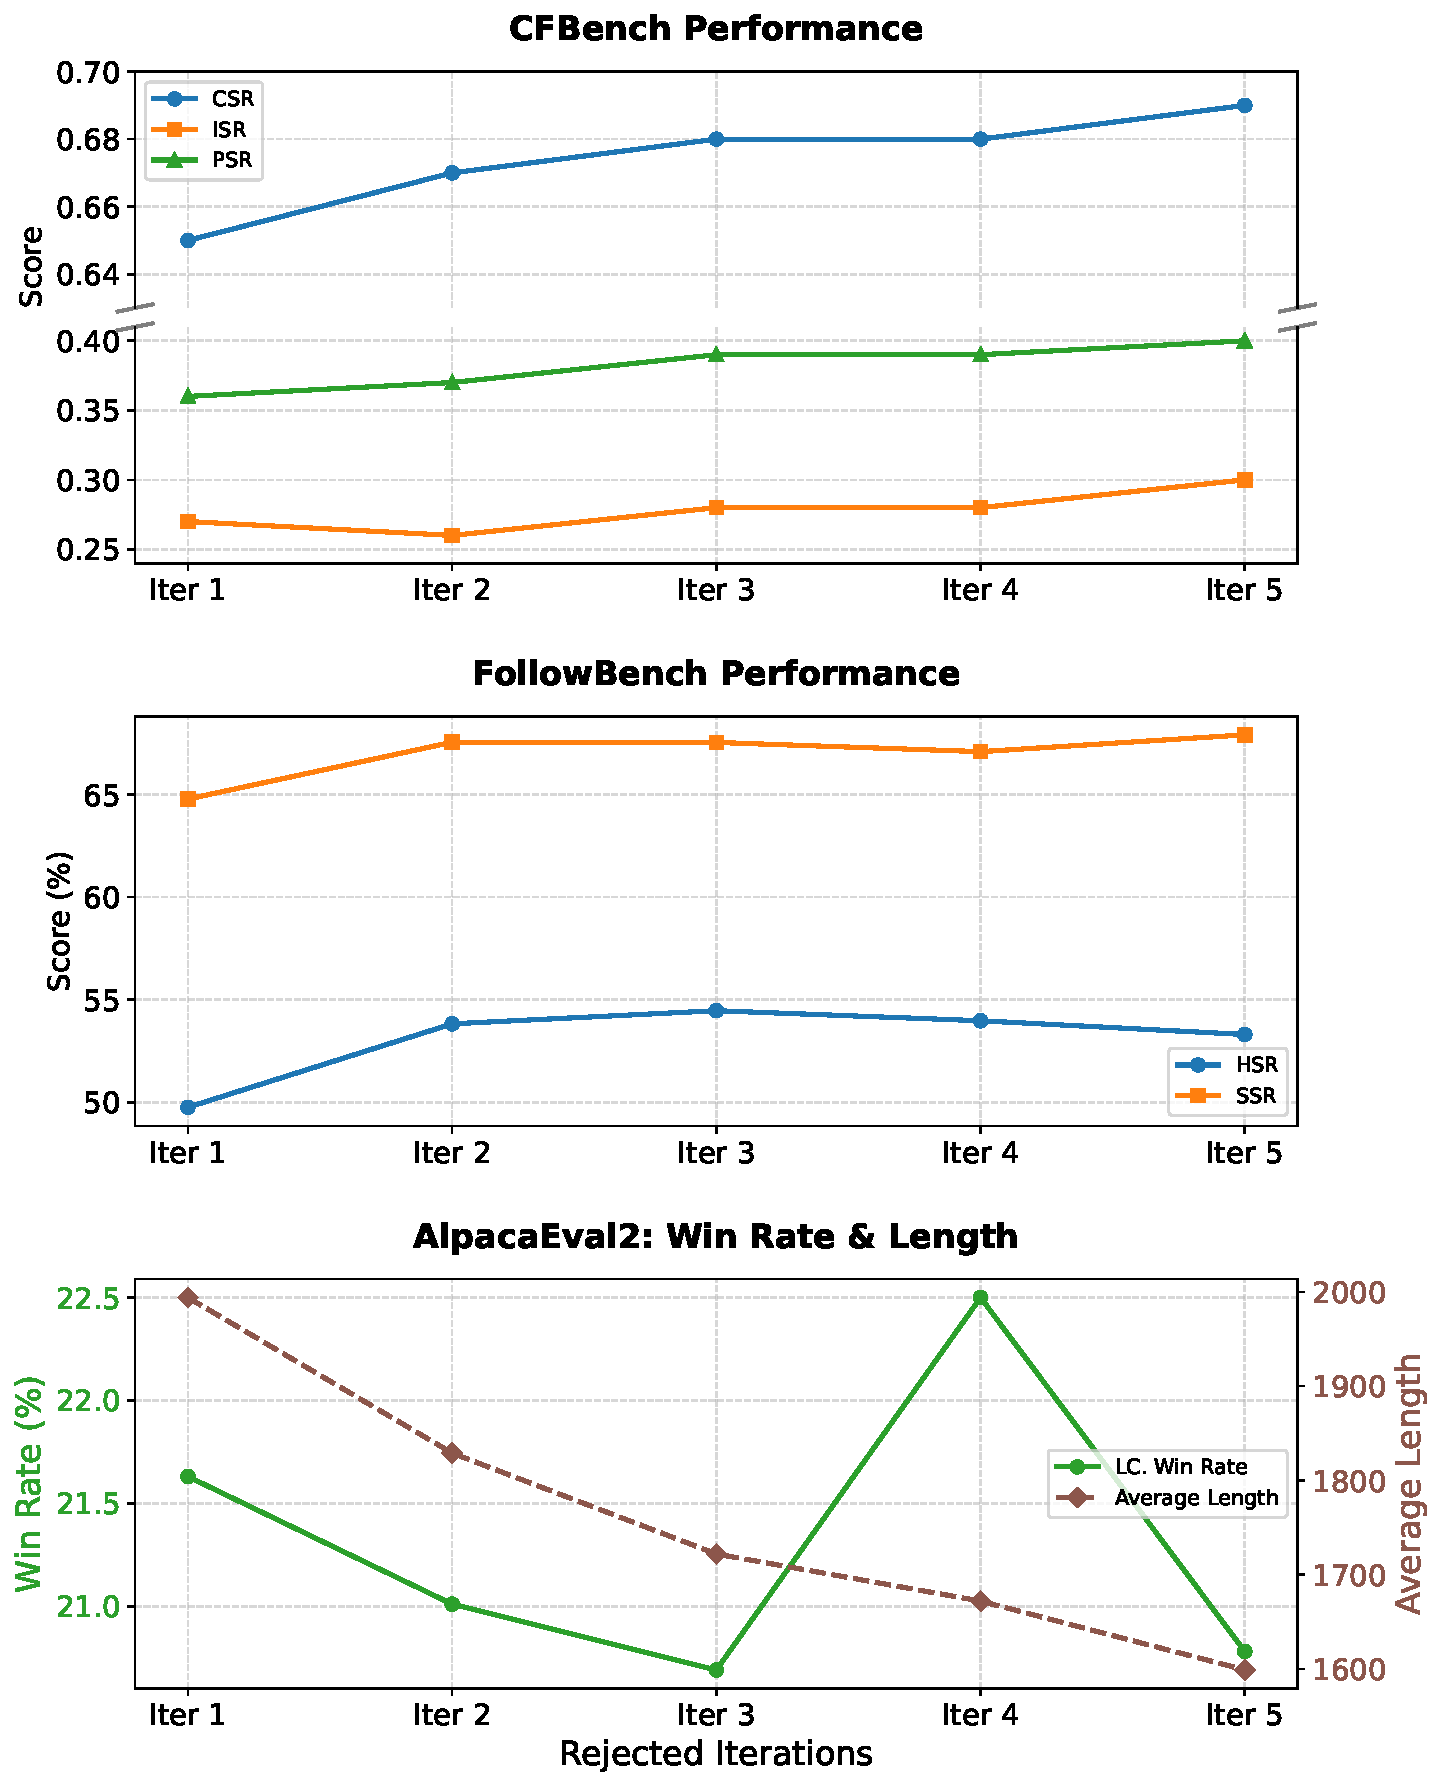
\includegraphics[width=0.48\textwidth]{source/sft_multi_turn.pdf}
    \caption{SFT performance with data from different iterations on Llama-3-8B-Tulu.}
    \label{figure:iterative_sft}
\end{figure}

As discussed in Section \ref{sec:IIR}, we apply multiple refinement iterations to ensure the quality of complex instructions. In this section, we investigate the effectiveness of our iterative refinement approach by measuring SFT model performance across different iterations. As shown in Figure \ref{figure:iterative_sft}, we evaluate SFT models trained on data from different iterations.

% and track the average input and output token counts to quantify the computational cost associated with each iteration.

% 下面这里增加了cfbench结果，画图代码在：source/sft_multi_turn_figure.py

Specifically, we observe consistent improvements on CFBench, FollowBench and AlpacaEval2 through the first two iterations. In particular, CFBench exhibits steady growth across all metrics. This suggests that the iterative judging process effectively identifies and incorporates increasingly sophisticated constraints that are valuable for complex instruction following. However, improvements tend to plateau after the third iteration. This could be attributed to the fact that the most critical and fundamental constraints for effective alignment have already been discovered in earlier iterations. Furthermore, we observe a steady decline in the average output length on AlpacaEval2. This indicates that the iteration process enhances alignment precision, enabling the model to provide more concise responses without unnecessary verbosity.

To verify that the benefits of iterative refinement do not stem simply from an increased number of constraints, we compared our method against a one-shot baseline, where multiple constraints are generated simultaneously without iteration. As shown in Table \ref{table:judge_iterations2}, the one-shot approach is less effective for SFT, as it lacks the progressive discovery process, which is crucial for uncovering challenging constraints with higher complexity (measured by Unique Trigrams).

% We further present computational cost analysis in Figure \ref{figure:instruction_and_complexity}. As can be seen, the metrics demonstrate a steady improvement of data quality as the iterations progress. While multiple iterations introduce additional computational overhead, they are crucial for generating more valuable constraints and improving the model's ability.

% 这个子图已经去掉了
% Moreover, as shown in Figure \ref{figure:instruction_and_complexity}, data quality improves steadily across iterations. Despite the increased computational costs reflected in Figure \ref{figure:iterative_sft}, where both input and output token numbers increase, requiring more computational resources for training, these iterations generate more valuable constraints that directly enhance model performance.

\begin{table}[!t]
\centering
\caption{SFT performance of 1-shot and 5-iteration instruction generation on Llama-3-8B-Tulu.}
\renewcommand{\arraystretch}{0.95}
\resizebox{0.48\textwidth}{!}{
\begin{tabular}{c|cc|cc|c}
\toprule
\multirow{2}{*}{\textbf{Method}} & \multicolumn{2}{c|}{\textbf{FollowBench}} & \multicolumn{2}{c|}{\textbf{AlpacaEval2}} & \multirow{2}{*}{\textbf{Uni-Trigrams}}
\\
& \textbf{HSR}        & \textbf{SSR}       & \textbf{LC.}      & \textbf{Len}  \\ 
\midrule
1-shot   & 50.17     & 63.82    & 18.49    & 1,566 & 41.72 \\
5-iteration	   & \textbf{53.30}     & \textbf{67.91}    & \textbf{20.78}    & 1,599  & 67.45 \\
\bottomrule
\end{tabular}}
\label{table:judge_iterations2}
\end{table}

\subsection{Influence of Iterative Refinement on RM Efficacy}

\begin{table*}[!t]
\centering
\caption{SFT performance with constraints from different judgment strategies on Llama-3-8B models (UltraChat and Tulu).}
\renewcommand{\arraystretch}{1.1}
\resizebox{0.85\textwidth}{!}{
\begin{tabular}{l|l|ccc|cc|cc}
\toprule
\multirow{2}{*}{\textbf{Base Model}} & \multirow{2}{*}{\textbf{Method}} & \multicolumn{3}{c}{\textbf{CF-Bench}} & \multicolumn{2}{c}{\textbf{FollowBench}} & \multicolumn{2}{c}{\textbf{AlpacaEval2}} \\
\cmidrule(lr){3-5} \cmidrule(lr){6-7} \cmidrule(lr){8-9}
& & \textbf{CSR} & \textbf{ISR} & \textbf{PSR} & \textbf{HSR} & \textbf{SSR} & \textbf{LC.} & \textbf{Len} \\
\midrule
\multirow{5}{*}{\makecell[l]{Llama-3-8B-UltraChat}} 
& Baseline & 0.51 & 0.15 & 0.22 & 41.04 & 57.39 & 8.86 & 1,017 \\
\cmidrule{2-9} % <--- 为 UltraChat 部分添加横线
& No Judge & 0.63 & 0.25 & 0.34 & 47.15 & 62.62 & 19.07 & 1,706 \\
& Document-free Judge & 0.62 & 0.25 & 0.34 & 51.24 & 63.81 & 20.00 & 1,717 \\
& \textbf{Document-based Judge} & \textbf{0.64} & \textbf{0.26} & \textbf{0.34} & \textbf{52.34} & \textbf{64.09} & 19.74 & 1,408 \\
& \quad + check & 0.61 & 0.24 & 0.31 & 50.69 & 63.89 & \textbf{21.00} & 1,813 \\
\midrule
\midrule
\multirow{5}{*}{\makecell[l]{Llama-3-8B-Tulu}} 
& Baseline & 0.50 & 0.15 & 0.20 & 34.91 & 51.76 & 5.20 & 995 \\
\cmidrule{2-9} % <--- 为 Tulu 部分添加横线
& No Judge & 0.66 & 0.28 & 0.38 & 47.59 & 63.60 & 18.32 & 2,067 \\
& Document-free Judge & 0.67 & 0.27 & 0.38 & 50.62 & 63.69 & 17.02 & 2,842 \\
& \textbf{Document-based Judge} & \textbf{0.67} & \textbf{0.27} & \textbf{0.38} & \textbf{54.16} & \textbf{67.52} & 20.45 & 1,639 \\
& \quad + check & 0.66 & 0.26 & 0.37 & 51.35 & 66.09 & \textbf{21.09} & 2,049 \\
\bottomrule
\end{tabular}}
\label{table:judge}
\end{table*}

\begin{figure}[pos=htbp]
    \centering
    \includegraphics[width=0.48\textwidth]{source/RM_iterations.png}
    \caption{RL performance with RM trained on rejected responses from different iterations on Llama-3-8B-UltraChat.}
    \label{figure:iterative_rm}
\end{figure}

As discussed in Section \ref{sec:rl}, we utilize responses generated from different iterations as rejected samples for RM training. To investigate how the gap between chosen and rejected samples influences RM efficacy, we trained multiple RMs by pairing a fixed set of chosen samples with rejected samples from varying iterations. These RMs were subsequently employed in RL training to evaluate their impact on alignment performance, as shown in Figure \ref{figure:iterative_rm}.

The results show that RL performance follows an inverted U-shaped trend as the iteration index of rejected samples increases. Utilizing responses from the second iteration as rejected samples yielded optimal performance across both complex and general benchmarks. Notably, the average output length on AlpacaEval2 decreased significantly with Iter 2, indicating that the model effectively suppressed verbosity while improving overall performance.

Using rejected samples from either too early or too late iterations leads to performance degradation. With later iterations (e.g., Iter 4-5), the quality of rejected samples improves to the point where they closely resemble chosen responses, narrowing the contrastive space and hindering the RM's ability to capture preference signals. Conversely, with earlier iterations (e.g., Iter 0-1), the gap between chosen and rejected samples is so large that the task becomes trivial, preventing the RM from learning to distinguish fine-grained quality differences. In summary, selecting rejected samples of moderate difficulty is crucial for ensuring RM's efficacy for the RL process.

\subsection{Judgment Strategy for Better Constraint}
\label{sec:judge}

% \begin{table}[!t]
% \centering
% \caption{Experiment results on Llama-3-8B models with constraints from different judgment strategies.}
% \renewcommand{\arraystretch}{0.95}
% \resizebox{0.44\textwidth}{!}{
% \begin{tabular}{c|cc|cc}
% \toprule
% \multirow{2}{*}{\textbf{Method}} & \multicolumn{2}{c|}{\textbf{FollowBench}} & \multicolumn{2}{c}{\textbf{AlpacaEval2}} \\
% & \textbf{HSR} & \textbf{SSR} & \textbf{LC.} & \textbf{Len} \\
% \midrule
% \multicolumn{5}{l}{\textit{Results on Llama-3-8B-UltraChat}} \\
% \midrule
% Baseline & 41.04 & 57.39 & 8.86 & 1,017 \\
% \midrule
% w/o judge & 47.15 & 62.62 & 19.07 & 1,706 \\
% judge w/o doc & 51.24 & 63.81 & 20.00 & 1,717 \\
% judge w/ doc & \textbf{52.34} & \textbf{64.09} & 19.74 & 1,408 \\
% \midrule
% w/ check & 50.69 & 63.89 & \textbf{21.00} & 1,813 \\
% \midrule
% \multicolumn{5}{l}{\textit{Results on Llama-3-8B-Tulu}} \\
% \midrule
% Baseline & 34.91 & 51.76 & 5.20 & 995 \\
% \midrule	
% w/o judge & 47.59 & 63.60 & 18.32 & 2,067 \\
% judge w/o doc & 50.62 & 63.69 & 17.02 & 2,842 \\
% judge w/ doc & \textbf{54.16} & \textbf{67.52} & 20.45 & 1,639 \\
% \midrule
% w/ check & 51.35 & 66.09 & \textbf{21.09} & 2,049 \\
% \bottomrule
% \end{tabular}}
% \label{table:judge}
% \end{table}

\begin{table}[!t]
\centering
\caption{SFT performance with different sampling strategies on Llama-3-8B-UltraChat .}
\renewcommand{\arraystretch}{0.95}
\resizebox{0.47\textwidth}{!}{
\begin{tabular}{c|cc|cc|c}
\toprule
\multirow{2}{*}{\textbf{Method}} & \multicolumn{2}{c|}{\textbf{FollowBench}} & \multicolumn{2}{c|}{\textbf{AlpacaEval2}} & \textbf{Unique} \\
& \textbf{HSR}        & \textbf{SSR}       & \textbf{LC.}      & \textbf{Len} & \textbf{Trigrams} \\ 
\midrule
Baseline  & 41.04       & 57.39      & 8.86       & 1,017 & - \\
\midrule
Random 1K    & 41.71   & 57.66    & 12.26  & 1,313 & 45.13 \\
Density 1K    & \textbf{45.85}   & \textbf{60.21}    & \textbf{17.15}  & 1,611 & \textbf{66.81} \\
InsTag 1K   & 44.11    & 59.89    & 13.03     & 1,251 & 58.09 \\
\bottomrule
\end{tabular}}
\label{table:sampling}
\end{table}

In this section, we investigate the optimal judgment strategy for constraint generation by comparing three distinct configurations: (1) No Judgment, where constraints are generated directly; (2) Document-free Judgment, which relies on the guidance model’s own response as the basis for new constraints; and (3) Document-based Judgment, which leverages the refined document as the reference for new constraints.

As shown in Table \ref{table:judge}, the iterative judgment process is indispensable for uncovering valuable constraints that enhance instruction-following capabilities. Notably, the Document-based Judgment setting achieves the best performance on both complex and general instruction benchmarks. This suggests that the refined document serves as a crucial gold standard, allowing the LLM-judge to pinpoint model deficiencies more accurately than when relying on self-generated, potentially flawed outputs. This mechanism mirrors human behavior: when users refine prompts based on model outputs, they typically hold an intrinsic reference in mind and issue constraints to guide the response toward that expectation.

Regarding the additional checking step (+ check), where generated constraints are further filtered based on their alignment with the model's eventual output, we observe a decline in complex instruction-following performance. This suggests that the checking mechanism may be overly restrictive, inadvertently filtering out subtle yet essential constraints that are necessary for precise instruction alignment. 

% However, this step improves performance on general instruction following on AlpacaEval2, revealing a trade-off: stricter constraint filtering favors general conversational fluency but is harmful for complex instruction adherence.

\begin{figure}[pos=htbp]
\centering
\includegraphics[width=0.48\textwidth]{source/llama_Tulu_DataNum.png}
\caption{SFT performance with different data volume on Llama-3-8B-Tulu.}
\label{figure:data_num}
\end{figure}

\begin{table*}[!t]
\centering
\caption{RL performance with different RM configurations on Llama-3-8B-UltraChat and Qwen-2.5-7B-UltraChat.}
% \setlength{\tabcolsep}{8pt}
\renewcommand{\arraystretch}{1.1}
\resizebox{0.85\textwidth}{!}{
\begin{tabular}{l|l|ccc|cc|cc}
\toprule
\multirow{2}{*}{\textbf{Base Model}} & \multirow{2}{*}{\textbf{Method}} & \multicolumn{3}{c}{\textbf{CF-Bench}} & \multicolumn{2}{c}{\textbf{FollowBench}} & \multicolumn{2}{c}{\textbf{AlpacaEval2}} \\
\cmidrule(lr){3-5} \cmidrule(lr){6-7} \cmidrule(lr){8-9}
& & \textbf{CSR} & \textbf{ISR} & \textbf{PSR} & \textbf{HSR} & \textbf{SSR} & \textbf{LC.} & \textbf{Len} \\
\midrule
\multirow{5}{*}{\makecell[l]{Llama-3-8B-UltraChat}} 
& Baseline & 0.51 & 0.15 & 0.22 & 41.04 & 57.39 & 8.86 & 1,017 \\
\cmidrule{2-9}
& DIR-SFT & 0.61 & 0.24 & 0.31 & 50.69 & 63.89 & 21.00 & 1,813 \\
& DIR-RL w/ RM-3B & 0.62 & 0.24 & 0.32 & 51.31 & 64.03 & 21.89 & 2,387 \\
& \textbf{DIR-RL w/ RM-8B} & \textbf{0.62} & \textbf{0.26} & \textbf{0.34} & \textbf{53.83} & \textbf{65.55} & \textbf{22.07} & 2,271 \\
& \quad w/o Rule-based Reward & 0.60 & 0.24 & 0.32 & 52.17 & 63.82 & 20.91 & 2,413 \\
\midrule
\midrule
\multirow{5}{*}{\makecell[l]{Qwen-2.5-7B-UltraChat}} 
& Baseline & 0.68 & 0.29 & 0.40 & 47.71 & 64.79 & 10.87 & 836 \\
\cmidrule{2-9}
& DIR-SFT & 0.76 & 0.41 & 0.51 & 59.07 & 71.35 & 32.43 & 1,779 \\
& DIR-RL w/ RM-3B & 0.76 & 0.43 & 0.53 & 60.04 & 72.57 & 33.00 & 2,109 \\
& \textbf{DIR-RL w/ RM-8B} & \textbf{0.77} & \textbf{0.45} & \textbf{0.54} & \textbf{62.53} & \textbf{72.68} & \textbf{35.49} & 1,988 \\
& \quad w/o Rule-based Reward & 0.74 & 0.42 & 0.51 & 59.94 & 70.10 & 32.88 & 2,179 \\
\bottomrule
\end{tabular}}
\label{table:rm-training}
\end{table*}

\subsection{Impact of SFT Configurations}

In this section, we investigate the impact of various SFT configurations on DIR's performance, focusing primarily on two key factors: the sampling strategy for document selection and the volume of training data.

As detailed in Section \ref{sec:document_collection}, we utilize density-based sampling to ensure the diversity of our document set. To verify the effectiveness of this approach, we compared it against two baselines for selecting SFT samples:

\begin{enumerate}[itemsep=1mm, parsep=0pt, leftmargin=*]
    \item \textbf{Random 1K}: Randomly selecting 1K samples.
    \item \textbf{Density 1K}: Selecting 1K samples using our proposed density-based sampling method.
    \item \textbf{InsTag 1K} \citep{Lu2023InsTagIT}: Using GPT-4\footnote{Specifically, we use GPT-4o-0806 for InsTag.} to label each instruction with semantic and complexity tags, then selecting instructions to ensure diverse representation.
\end{enumerate}

As shown in Table \ref{table:sampling}, our density-based method significantly outperforms both random selection and InsTag across complex and general instruction-following benchmarks. Notably, despite the high computational cost associated with InsTag's LLM-based tagging process, InsTag yields lower performance than our approach. We also analyzed the lexical diversity of the sampled instructions by calculating the average unique trigrams. The results indicate that our method selects more diverse samples (66.81 unique trigrams), which correlates with the superior downstream performance.

We further analyze the relationship between training data volume and SFT performance in Figure \ref{figure:data_num}. As can be seen, performance on both general and complex instruction benchmarks scales positively with the amount of training data, underscoring the scalability of the DIR framework. On the other hand, the model can achieve superior performance with only 1K training samples, highlighting the efficiency of our data synthesis process in minimizing SFT overhead.

\subsection{Impact of RM Configurations}

To investigate the impact of RM configurations on downstream RL performance, we conduct ablation studies on model scale and the integration of rule-based reward signals. Table \ref{table:rm-training} presents a comparative analysis between RMs initialized from Llama-3.2-3B and Llama-3.1-8B, evaluating their effectiveness with and without rule-based components.

Our results demonstrate a positive correlation between RM scale and feedback quality. Across RL experiments on different policy models, the 8B-scale RM consistently outperforms its 3B counterpart. This performance gap likely stems from the superior linguistic nuances and logical reasoning inherent in larger base models, allowing the 8B RM to capture more sophisticated preference signals to guide policy optimization.

Furthermore, incorporating rule-based reward signals proved essential, and removing these signals led to a marked performance decline across both complex and general instruction benchmarks. For instruction alignment, verifiable constraints (e.g., formatting, keywords) provide deterministic, low-noise feedback. By establishing a rigid correspondence between constraints and outputs, these signals significantly accelerate convergence during constraint-aware RL.

% \begin{table*}[!ht]
% \centering
% \caption{Experiment results on Llama-3-8B and Qwen-2.5-7B, with both models fine-tuned with ultrachat-200k. Llama-3-70B-Instruct and Qwen-2.5-72B-Instruct are used as the guidance models respectively.}
% \setlength{\tabcolsep}{12pt}
% \renewcommand{\arraystretch}{0.9}
% \resizebox{0.98\textwidth}{!}{
% \begin{tabular}{l|ccc|cc|cc}
% \toprule
% \multicolumn{8}{c}{\textbf{Fine-tuned on Llama-3-8B-UltraChat}} \\
% \midrule
% \multirow{2}{*}{\textbf{Method}} & \multicolumn{3}{c}{\textbf{CFBench}} & \multicolumn{2}{c}{\textbf{FollowBench}} & \multicolumn{2}{c}{\textbf{AlpacaEval2}} \\
% \cmidrule(lr){2-4} \cmidrule(lr){5-6} \cmidrule(lr){7-8}
% & \textbf{CSR} & \textbf{ISR} & \textbf{PSR} & \textbf{HSR} & \textbf{SSR} & \textbf{LC.} & \textbf{Len} \\
% \midrule
% Baseline & 0.51 & 0.15 & 0.22 & 41.04 & 57.39 & 8.86 & 1,017 \\
% DIR-SFT & 0.61 & 0.24 & 0.31 & 50.69 & 63.89 & 21.00 & 1,813 \\
% DIR-RL w/ RM-3B & 0.62 & 0.24 & 0.32 & 51.31 & 64.03 & 21.89 & 2,387 \\
% DIR-RL w/ RM-8B & 0.62 & 0.26 & 0.34 & 53.83 & 65.55 & 22.07 & 2,271 \\
% w/o Rule-based Reward & 0.60 & 0.24 & 0.32 & 52.17 & 63.82 & 20.91 & 2,413 \\
% \midrule
% \midrule
% \multicolumn{8}{c}{\textbf{Fine-tuned on Qwen-2.5-7B-UltraChat}} \\
% \midrule
% \multirow{2}{*}{\textbf{Method}} & \multicolumn{3}{c}{\textbf{CFBench}} & \multicolumn{2}{c}{\textbf{FollowBench}} & \multicolumn{2}{c}{\textbf{AlpacaEval2}} \\
% \cmidrule(lr){2-4} \cmidrule(lr){5-6} \cmidrule(lr){7-8}
% & \textbf{CSR} & \textbf{ISR} & \textbf{PSR} & \textbf{HSR} & \textbf{SSR} & \textbf{LC.} & \textbf{Len} \\
% \midrule
% Baseline & 0.68 & 0.29 & 0.40 & 47.71 & 64.79 & 10.87 & 836 \\
% DIR-SFT & 0.76 & 0.41 & 0.51 & 59.07 & 71.35 & 32.43 & 1,779 \\
% DIR-RL w/ RM-3B & 0.76 & 0.43 & 0.53 & 60.04 & 72.57 & 33.00 & 2,109 \\
% DIR-RL w/ RM-8B & 0.77 & 0.45 & 0.54 & 62.53 & 72.68 & 35.49 & 1,988 \\
% w/o Rule-based Reward & 0.74 & 0.42 & 0.51 & 59.94 & 70.10 & 32.88 & 2,179 \\
% \bottomrule
% \end{tabular}}
% \label{table:rm-training}
% \end{table*}

% \begin{table*}[!ht]
% \centering
% \caption{Main results on Llama-3-8B-UltraChat. We evaluate the performance across CF-Bench, FollowBench, and AlpacaEval2. The best results are highlighted in bold.}
% \setlength{\tabcolsep}{12pt}
% \renewcommand{\arraystretch}{0.9}
% \resizebox{0.98\textwidth}{!}{
% \begin{tabular}{l|ccc|cc|cc}
% \toprule
% \multicolumn{8}{c}{\multirow{2}{*}{\raisebox{1.4em}{\makecell{\textbf{Fine-tuned on Llama-3-8B-UltraChat}}}}} \\
% \midrule
% \multirow{2}{*}{\raisebox{-0.4em}{\textbf{Method}}} & \multicolumn{3}{c}{\textbf{CF-Bench}}      & \multicolumn{2}{c}{\textbf{FollowBench}} & \multicolumn{2}{c}{\textbf{AlpacaEval2}} \\
% \cmidrule(lr){2-4} \cmidrule(lr){5-6} \cmidrule(lr){7-8}
% & \textbf{CSR} & \textbf{ISR} & \textbf{PSR} & \textbf{HSR}        & \textbf{SSR}       & \textbf{LC.}        & \textbf{Len}        \\
% \midrule
% Baseline    & 0.51         & 0.15         & 0.22         & 41.04               & 57.39              & 8.86                & 1,017               \\ 
% \midrule
% DIR-SFT     & 0.61         & 0.24         & 0.31         & 50.69               & 63.89              & 21.00               & 1,813               \\
% \textbf{GRPO (Ours)} & \textbf{0.62} & \textbf{0.26} & \textbf{0.34} & \textbf{53.83}      & \textbf{65.55}     & \textbf{22.07}      & 2,271               \\
% \quad w/o KL Removal & 0.61         & 0.25         & 0.33         & 53.15               & 65.09              & 21.84               & 2,143               \\
% \quad w/o Dynamic Sampling & 0.61         & 0.25         & 0.32         & 52.47               & 64.66              & 21.52               & 2,118               \\
% \midrule
% PPO         & 0.59         & 0.24         & 0.31         & 53.02               & 64.84              & 21.95               & 1,945               \\
% Reinforce++ & 0.59         & 0.23         & 0.31         & 51.96               & 63.71              & 20.88               & 2,629               \\
% \bottomrule
% \end{tabular}}
% \label{table:ablation_no_green}
% \end{table*}

\begin{table*}[!t]
\centering
\caption{Experiment results of different RL methods with RM-8B on Llama-3-8B-UltraChat.}
\renewcommand{\arraystretch}{1.1}
\resizebox{0.85\textwidth}{!}{
\begin{tabular}{l|l|ccc|cc|cc}
\toprule
\multirow{2}{*}{\textbf{Base Model}} & \multirow{2}{*}{\textbf{Method}} & \multicolumn{3}{c}{\textbf{CF-Bench}}      & \multicolumn{2}{c}{\textbf{FollowBench}} & \multicolumn{2}{c}{\textbf{AlpacaEval2}} \\
\cmidrule(lr){3-5} \cmidrule(lr){6-7} \cmidrule(lr){8-9}
& & \textbf{CSR} & \textbf{ISR} & \textbf{PSR} & \textbf{HSR}        & \textbf{SSR}       & \textbf{LC.}        & \textbf{Len}        \\
\midrule
\multirow{7}{*}{\makecell[l]{Llama-3-8B-UltraChat}} 
& Baseline    & 0.51         & 0.15         & 0.22         & 41.04               & 57.39              & 8.86                & 1,017               \\ 
\cmidrule(lr){2-9}
& DIR-SFT     & 0.61         & 0.24         & 0.31         & 50.69               & 63.89              & 21.00               & 1,813               \\
& \textbf{DIR-RL (GRPO)} & \textbf{0.62} & \textbf{0.26} & \textbf{0.34} & \textbf{53.83}      & \textbf{65.55}     & \textbf{22.07}      & 2,271               \\
& \quad w/o KL Relaxation & 0.61         & 0.25         & 0.33         & 53.15               & 65.09              & 21.84               & 2,143               \\
& \quad w/o Dynamic Sampling & 0.61         & 0.25         & 0.32         & 52.47               & 64.66              & 21.52               & 2,118               \\
\cmidrule(lr){2-9}
& PPO         & 0.59         & 0.24         & 0.31         & 53.02               & 64.84              & 21.95               & 1,945               \\
% Reinforce++重训了一遍
& Reinforce++ & 0.61   & 0.25 & 0.33  & 53.54 & 65.26  & 21.76 & 2,403   \\
\bottomrule
\end{tabular}}
\label{table:ablation_rl}
\end{table*}

\subsection{Influence of RL Settings}

During the RL training phase, we implemented two key enhancements to the standard GRPO: KL-Penalty Relaxation and a Dynamic Sampling Mechanism. As shown in Table \ref{table:ablation_rl}, we conducted ablation studies to evaluate the effectiveness of these improvements and compared our method with other online reinforcement learning algorithms beyond GRPO.

Our results demonstrate that both of the two modifications are essential for instruction alignment. Specifically, KL-Penalty Relaxation unlocks the model's potential for hard-constraint tasks, while Dynamic Sampling ensures high-quality gradient updates. Consequently, the model achieves better performance across both complex and general benchmarks when both enhancements are integrated.

Furthermore, our improved GRPO consistently outperforms other popular RL algorithms such as PPO \citep{schulman2017proximal} and Reinforce++ \citep{hu2025reinforce++} under identical reward configurations. Unlike PPO, which often suffers from value estimation bias due to the difficulty of accurately predicting absolute rewards, GRPO leverages group-relative rewards which aligns more effectively with complex instruction tasks where response quality is inherently relative. Additionally, by employing intra-group normalization, GRPO enhances diversity and reduces gradient variance. This self-calibration allows GRPO to capture sparse reward signals more efficiently than Reinforce++, ultimately achieving better alignment performance.

% \begin{figure}[t]
% \centering
% \subfigure[Llama-3-8B-UltraChat]{
%     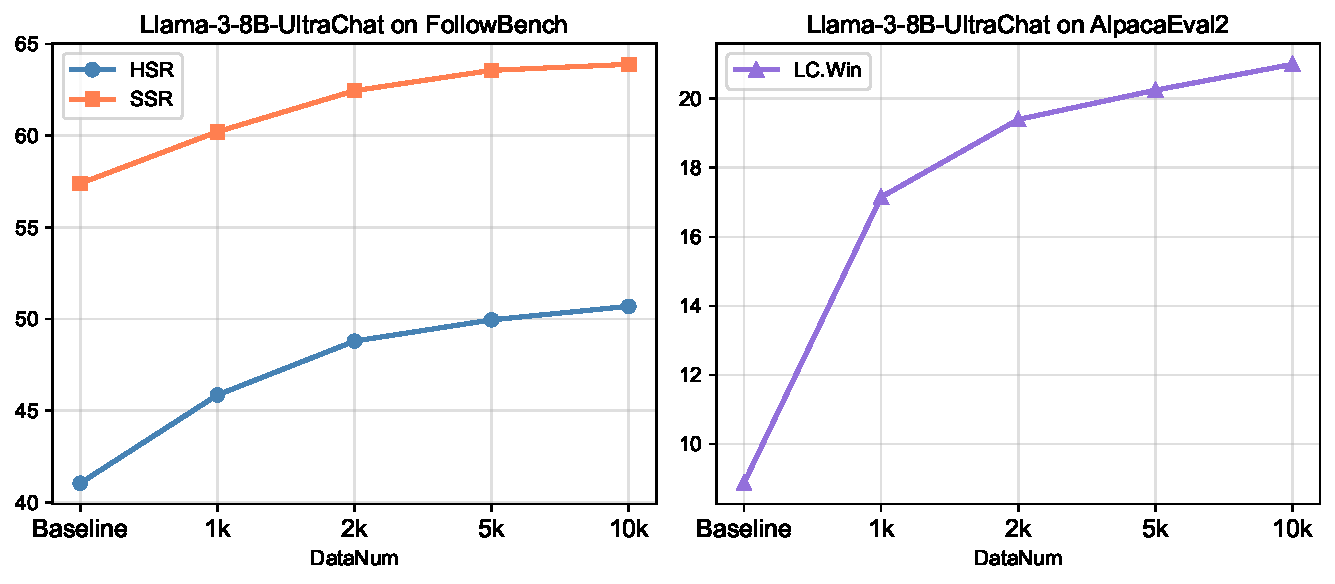
\includegraphics[width=0.95\linewidth]{source/data_visualization/llama_UltraChat_DataNum.pdf}
% }
% \subfigure[Llama-3-8B-Tulu]{
%     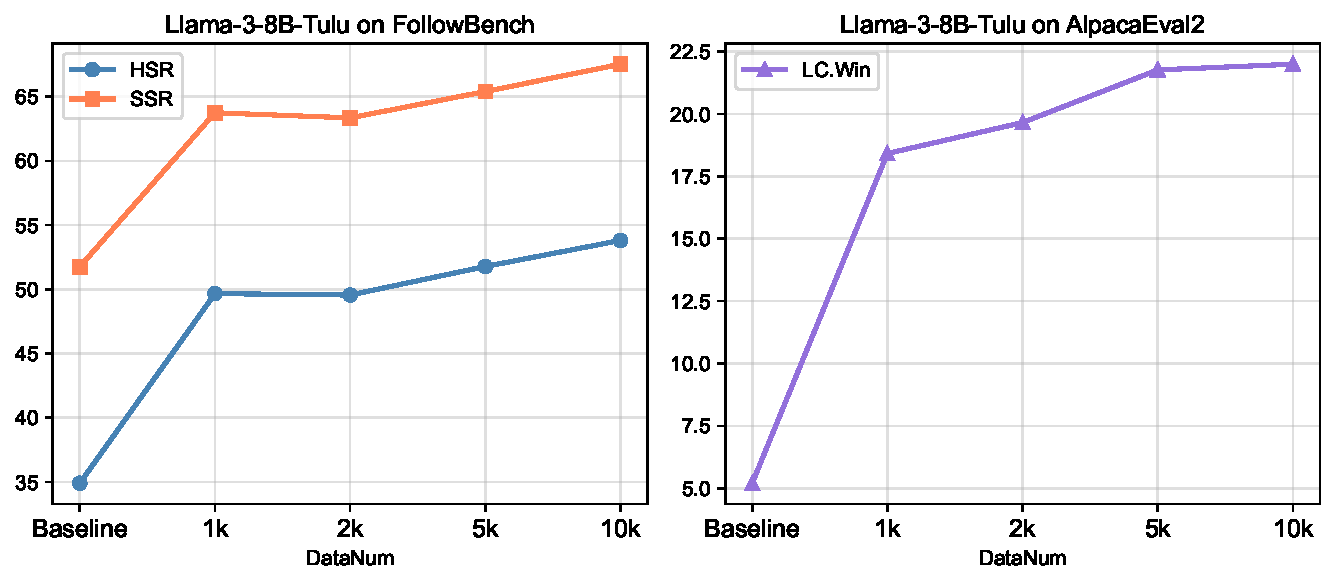
\includegraphics[width=0.95\linewidth]{source/data_visualization/llama_Tulu_DataNum.pdf}
% }
% \vspace{-3mm}
% \caption{The variation of performance on FollowBench and AlpacaEval2 with the variation of data number.}
% \vspace{-3mm}
% \label{figure:data_num}
% \end{figure}

\subsection{Impact on Fundamental Capabilities}

Previous methods have indicated LLMs may suffer from capability degradation during preference alignment phase, which is also known as alignment tax ~\citep{ouyang2022training}. To evaluate this concern, we tested our DIR method on several fundamental capability benchmarks: 1) World Knowledge: MMLU \citep{hendrycks2021measuring}; 2) Commonsense Reasoning: CommonsenseQA (CQA) \citep{talmor-etal-2019-commonsenseqa} and Natural Questions (NQ) \citep{kwiatkowski2019natural}; 3) Coding: HumanEval \citep{chen2021evaluatinglargelanguagemodels}; and 4) Mathematics: GSM8K \citep{cobbe2021trainingverifierssolvemath}. 

\begin{figure*}[pos=tbp]
\centering
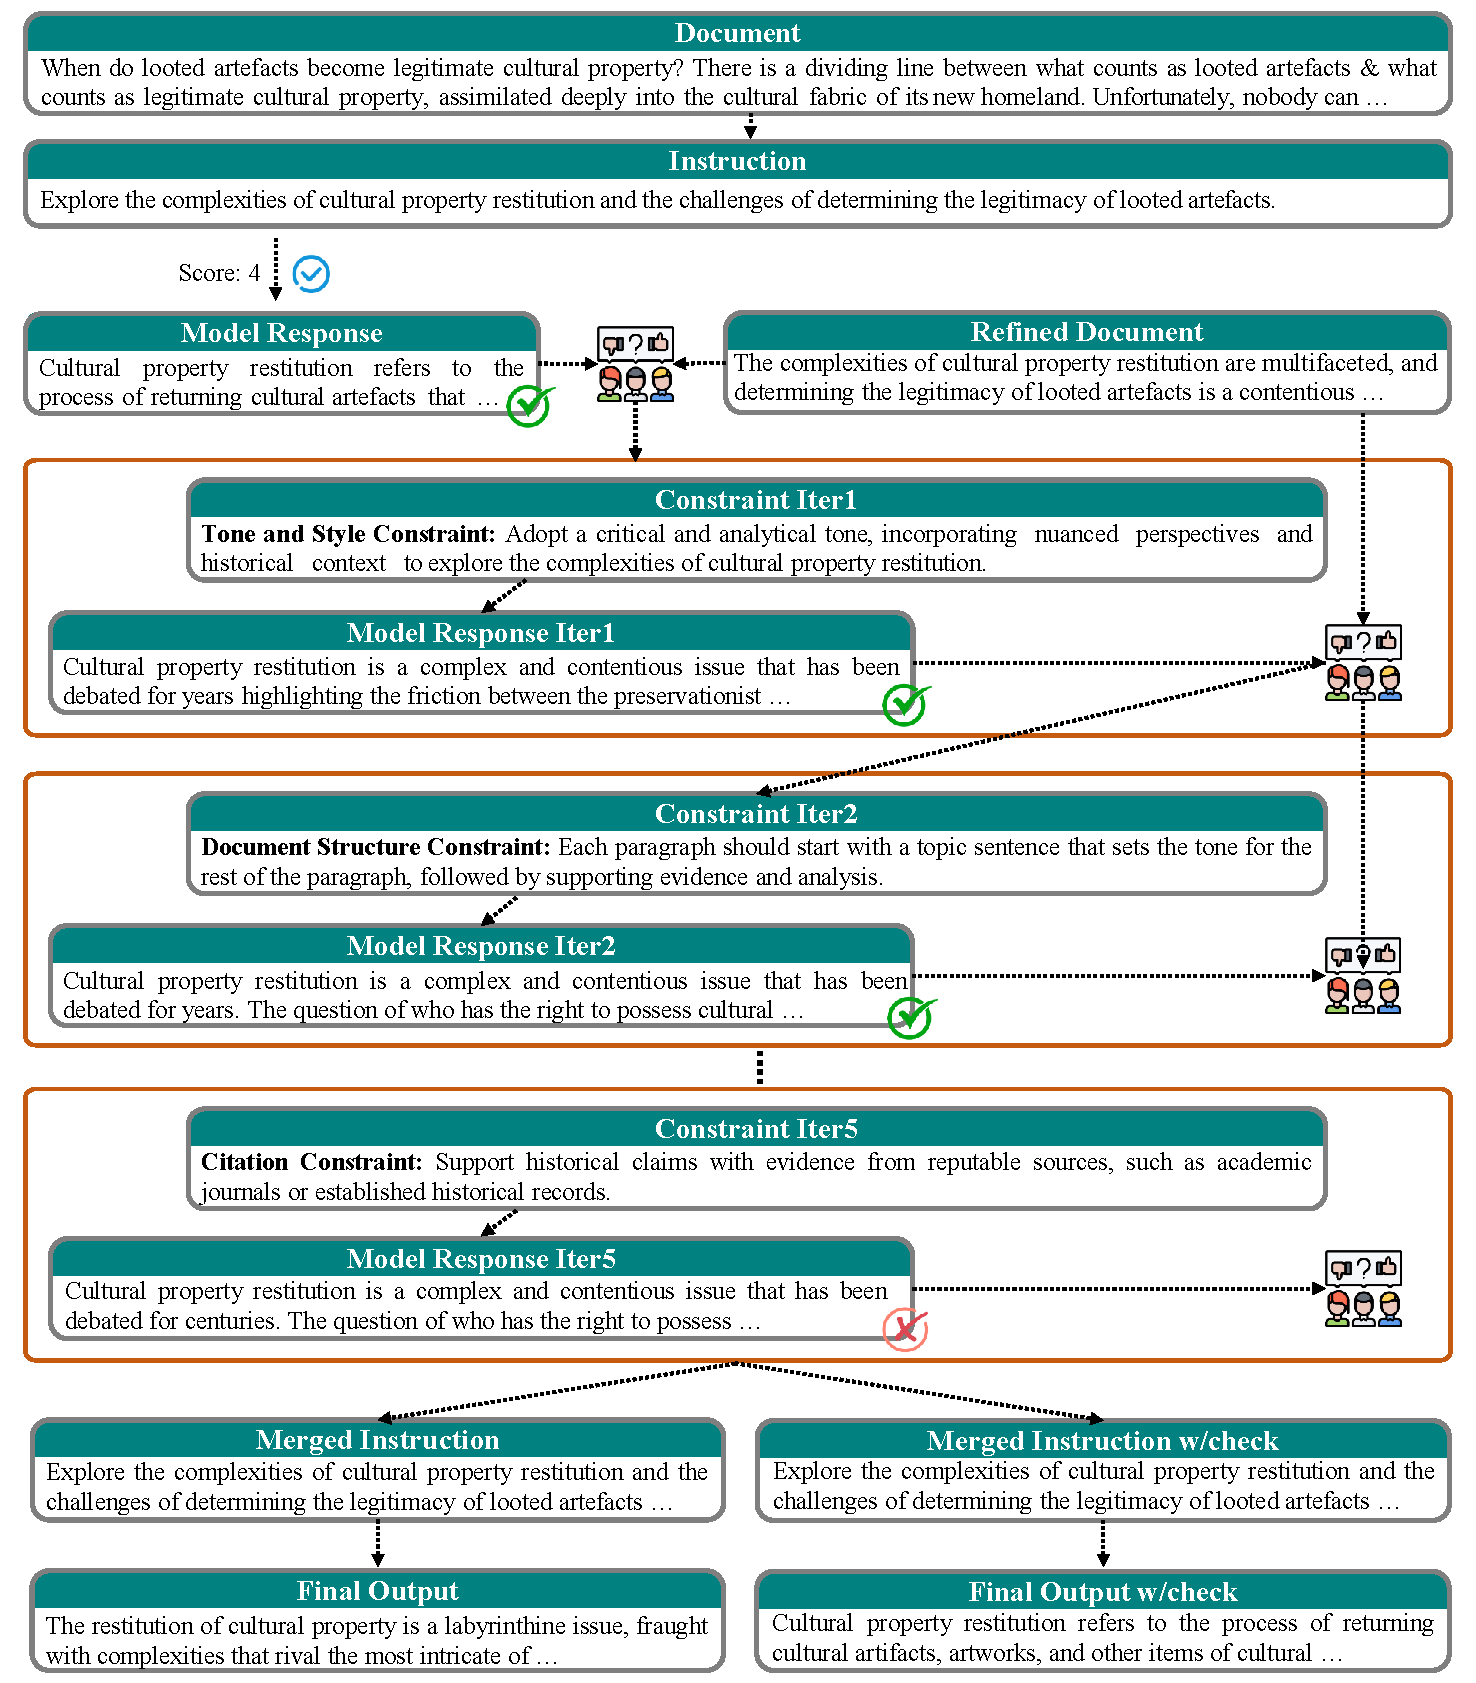
\includegraphics[width=0.88\linewidth]{source/pipeline_demo.pdf}
\caption{An End-to-End Document-grounded Iterative Refinement Example.}
\label{figure:pipeline_case}
\end{figure*}

\begin{table*}[t]
\centering
\caption{Evaluation results of fundamental capabilities of models optimized by DIR.}
\renewcommand{\arraystretch}{0.95}
\resizebox{0.8\textwidth}{!}{
\begin{tabular}{l|l|ccccc|c}
\toprule
\textbf{Base Model} & \textbf{Method} & \textbf{MMLU} & \textbf{CQA} & \textbf{NQ} & \textbf{HumanEval} & \textbf{GSM8K} & \textbf{AVG} \\
\midrule
\multirow{3}{*}{Llama-3-8B-UltraChat} 
& Baseline & 64.00 & 72.97 & 29.61 & 30.49 & 57.47 & 50.90 \\
& DIR-SFT & 61.64 & 73.63 & 30.54 & 29.88 & 54.59 & 50.05 \\
& DIR-RL & 63.48 & 74.15 & 31.27 & 29.53 & 58.29 & \textbf{51.34} \\
\midrule
\multirow{2}{*}{Qwen-2.5-7B-UltraChat} 
& Baseline & 73.64 & 82.39 & 25.68 & 52.20 & 81.65 & 63.11 \\
& DIR-SFT & 73.35 & 82.56 & 25.76 & 55.49 & 84.38 & 64.30 \\
& DIR-RL & 73.51 & 83.42 & 25.23 & 56.68 & 85.51 & \textbf{64.87} \\
\midrule
\multirow{2}{*}{Llama-3-8B-Tulu} 
& Baseline & 65.43 & 79.44 & 32.22 & 50.61 & 64.14 & 58.36 \\
& DIR-SFT & 64.95 & 79.92 & 34.62 & 50.85 & 63.70 & \textbf{58.80} \\
& DIR-RL & 64.27 & 79.13 & 31.56 & 51.18 & 63.41 & 57.91  \\
\bottomrule
\end{tabular}}
\label{table:fundamental}
\end{table*}

As shown in Table \ref{table:fundamental}, our method does not have a negative impact on fundamental capabilities. Specifically, DIR-RL improves the average performance of Llama-3-8B-UltraChat and Qwen-2.5-7B-UltraChat by 0.44 and 1.76 points, respectively. Similarly, DIR-SFT shows improvements on Qwen-2.5-7B-UltraChat and Llama-3-8B-Tulu by 1.19 and 0.44 points. This indicates that instructions synthesized from documents with evenly sampled distributions also exhibit even distribution, which is helpful for maintaining the fundamental knowledge and capabilities acquired during pre-train stage.

% \subsection{Robustness to Document Quality}

% \begin{table}[t]
% \centering
% \caption{Comparison of model performance when fine-tuned on instructions from different document sets.}
% \renewcommand{\arraystretch}{1.0}
% \resizebox{0.48\textwidth}{!}{
% \begin{tabular}{c|ccc|cc|cc}
% \toprule
% \multirow{2}{*}{\textbf{Data}} & \multicolumn{3}{c|}{\textbf{CFBench}} & \multicolumn{2}{c|}{\textbf{FollowBench}} & \multicolumn{2}{c}{\textbf{AlpacaEval2}} \\
% & \textbf{CSR} & \textbf{ISR} & \textbf{PSR} & \textbf{HSR} & \textbf{SSR} & \textbf{LC.} & \textbf{Len} \\
% \midrule
% random 1k & 0.61	& 0.23	& 0.33	& 45.85	& 60.21	& 17.15	& 1,611 \\
% low-quality 1k	& 0.60	& 0.22	& 0.30	& 44.00	& 59.83	& 16.10	& 1,685 \\
% \bottomrule
% \end{tabular}}
% \label{table:Robustness}
% \end{table}

% As discussed in Section \ref{sec:IIR}, our framework primarily utilizes documents to extract constraints rather than as direct fine-tuning targets. During fine-tuning, we use outputs from the guidance model as targets, which insulates the process from document quality issues. Moreover, we implemented multiple safeguards in our data production pipeline, which provides inherent robustness against document noise.

% To empirically validate our method's robustness to document quality, we conducted an additional experiment comparing two document sets: (1) a "low-quality" subset comprising the 1,000 lowest-scoring documents from DIR-10k (evaluated by GPT-4 across helpfulness, completeness, and harmlessness dimensions), and (2) a randomly sampled set of 1,000 documents from the same corpus.

% Table \ref{table:Robustness} presents the performance comparison of Llama-3-8B-UltraChat models fine-tuned on instructions derived from these two document sets. The results demonstrate negligible performance differences across all evaluation benchmarks. This empirical evidence confirms that our method maintains consistent performance regardless of input document quality, validating its robustness.

% Additionally, we provide the number of samples at each stage of the iterative process. As shown in Table \ref{table:Efficiency}, despite starting with a large number of initial documents, only 15\% of them are retained for iterative instruction refinement. Furthermore, nearly 50\% of the documents are filtered out during the iterations, leaving only the highest-quality samples for final training. This demonstrates how our carefully designed strategies effectively maintain sample quality across multiple iterations.

% \begin{table}[t]
% \centering
% \caption{Progressive reduction in sample size through filtering stages and five iterations.}
% \renewcommand{\arraystretch}{0.95}
% \resizebox{0.4\textwidth}{!}{
% \begin{tabular}{c|c}
% \toprule
% \textbf{Stage} & \textbf{Sample Number}\\
% \midrule
% Rule-based Filtering & 300k \\
% Density-based Sampling	& 60k \\
% Instruction Scoring	& 20k \\
% Iteration 1	& 17.3k \\
% Iteration 2	& 15.2k \\
% Iteration 3	& 13.7k \\
% Iteration 4	& 12.7k \\
% Iteration 5	& 11.9k \\
% \bottomrule
% \end{tabular}}
% \label{table:Efficiency}
% \end{table}

% \subsection{Influence of Guidance Model Size}
% \label{sec:Guidance_Model_Size}

% \begin{table}[!t]
% \centering
% \caption{Experiment results on Qwen-2.5-7B-UltraChat fine-tuned with different guidance model size.}
% \renewcommand{\arraystretch}{0.95}
% \resizebox{0.4\textwidth}{!}{
% \begin{tabular}{c|cc|cc}
% \toprule
% \multirow{2}{*}{\textbf{Guid. Model}} & \multicolumn{2}{c}{\textbf{FollowBench}} & \multicolumn{2}{c}{\textbf{AlpacaEval2}} \\
% & \textbf{HSR}   & \textbf{SSR}   & \textbf{LC.}      & \textbf{Len}  \\
% \midrule
% \begin{tabular}[c]{@{}c@{}}Baseline\end{tabular}  & 47.71    & 64.79  & 10.87   & 836   \\
% \midrule
% 14B     & 57.72   & 70.59   & 29.13   & 1,501   \\
% 32B     & \textbf{60.06}   & \textbf{71.97}   & 26.39   & 1,309    \\
% 72B     & 59.07   & 71.35   & \textbf{32.43}  & 1,779     \\
% \bottomrule
% \end{tabular}}
% \label{table:guidance_size}
% \end{table}

% In Table \ref{table:guidance_size}, we investigate the impact of guidance model size on DIR's performance. We performed experiments with Qwen-2.5-7B-UltraChat as the base model, while varying the guidance model size from 14B to 72B parameters. As shown, all guidance models with different sizes significantly improve instruction-following ability compared to the baseline, while larger models generally provide greater improvement. On the other hand, even the 14B guidance model demonstrates remarkable improvement. This scalability across different model sizes highlights the robustness and efficiency of our proposed approach.

% which leverages documents as reference to help the constraint generation process.

% These findings suggest that DIR's effectiveness is not strictly dependent on large guidance models. The method effectively leverages both document knowledge and model knowledge through judging mechanism to generate meaningful constraints, making it practical and efficient even with relatively smaller guidance models. 

\subsection{Case Study}

% This section presents a detailed end-to-end demonstration of our pipeline in Figure \ref{figure:pipeline_case}. The case study provides a thorough walkthrough of each stage in our instruction generation and refinement process.

To intuitively demonstrate how the DIR framework transforms unstructured documents into high-quality complex instructions, we provide an end-to-end example in Figure \ref{figure:pipeline_case}. As shown, through the document-grounded iterative refinement process, a complex instruction incorporating multifaceted constraints, including tone, structure, and citation requirements, is ultimately synthesized. This demonstrates that the DIR framework can effectively mine implicit human preferences within documents and transform them into explicit complex alignment signals.